\documentclass[aspectratio=169,10pt]{ctexbeamer}

\usetheme{Madrid}
\usecolortheme{default}
\usepackage{amsmath,amssymb,mathtools}
\usepackage{booktabs,tabularx}
\usepackage{graphicx}
\usepackage{tikz}
\usetikzlibrary{arrows.meta,positioning,fit}

\definecolor{mainblue}{RGB}{48,91,145}
\definecolor{accentorange}{RGB}{205,102,52}
\definecolor{goodgreen}{RGB}{54,132,86}
\definecolor{alertred}{RGB}{177,62,62}
\setbeamercolor{structure}{fg=mainblue}
\setbeamercolor{alerted text}{fg=alertred}
\setbeamercolor{block title}{bg=mainblue!15,fg=mainblue!80!black}
\setbeamercolor{block body}{bg=mainblue!4}
\setbeamercolor{exampleblock title}{bg=goodgreen!18,fg=goodgreen!65!black}
\setbeamercolor{exampleblock body}{bg=goodgreen!4}
\setbeamertemplate{navigation symbols}{}
\setbeamertemplate{caption}[numbered]
\setbeamertemplate{footline}{%
  \leavevmode%
  \hbox{%
    \begin{beamercolorbox}[wd=.78\paperwidth,ht=2.5ex,dp=1.1ex,leftskip=1em]{author in head/foot}%
      C.3 机器学习数据获取与数据定价
    \end{beamercolorbox}%
    \begin{beamercolorbox}[wd=.22\paperwidth,ht=2.5ex,dp=1.1ex,rightskip=1em plus1fil]{date in head/foot}%
      \insertframenumber/\inserttotalframenumber
    \end{beamercolorbox}%
  }%
}

\graphicspath{{../results/figures/}}
\newcommand{\E}{\mathbb E}
\newcommand{\Q}{\mathcal Q}
\newcommand{\Th}{\Theta}

\title{机器学习数据获取与数据定价}
\subtitle{Optimal Pricing for Data-Augmented AutoML Marketplaces\\论文讲解与缩减复现}
\author{课程大作业 C.3｜课程展示}
\date{2026年7月｜项目版本 v0.4.0}

\begin{document}

\begin{frame}
  \titlepage
\end{frame}

\begin{frame}{这篇论文解决什么问题？}
\begin{columns}[T,onlytextwidth]
\column{0.49\textwidth}
\begin{block}{现实矛盾}
\begin{itemize}
  \item 买家有 ML 任务，但训练数据少
  \item 平台拥有大量可连接的外部数据
  \item 原始数据价值难以事前判断、难以直接定价
\end{itemize}
\end{block}
\column{0.49\textwidth}
\begin{exampleblock}{论文的核心想法}
\begin{itemize}
  \item 联合搜索\textbf{外部数据增强 + ML 模型}
  \item 持续向买家展示当前模型性能
  \item 按可测量的模型性能/效用定价
  \item 买家自主决定继续搜索或停止
\end{itemize}
\end{exampleblock}
\end{columns}
\vspace{0.5em}
\centering
\large 数据获取与数据定价不再是两个独立问题
\end{frame}

\begin{frame}{市场工作流：从买家数据到价格曲线}
\centering
\begin{tikzpicture}[
  node distance=0.55cm and 0.36cm,
  box/.style={rounded corners,draw=mainblue,thick,fill=mainblue!6,
              minimum height=1.25cm,text width=2.12cm,align=center,font=\small},
  decision/.style={rounded corners,draw=accentorange,thick,fill=accentorange!7,
                   minimum height=1.25cm,text width=2.05cm,align=center,font=\small},
  arrow/.style={-{Latex[length=2.2mm]},thick,draw=gray!75}
]
\node[box] (buyer) {买家提交\\训练数据与任务};
\node[box,right=of buyer] (augment) {平台搜索\\外部增强数据};
\node[box,right=of augment] (model) {联合搜索\\模型/超参数};
\node[box,right=of model] (metric) {揭示当前性能\\$q_t\in\mathcal Q$};
\node[decision,right=of metric] (stop) {买家决策\\停止 / 继续};
\draw[arrow] (buyer)--(augment);
\draw[arrow] (augment)--(model);
\draw[arrow] (model)--(metric);
\draw[arrow] (metric)--(stop);
\draw[arrow,bend left=32] (stop.north) to node[above,font=\small]{继续，支付发现成本} (augment.north);
\node[box,below=0.8cm of stop] (purchase) {购买已发现模型\\支付 $x(q)$};
\draw[arrow] (stop)--node[right,font=\small]{停止}(purchase);
\end{tikzpicture}

\vspace{0.8em}
平台设计的是统一价格曲线 $x:\mathcal Q\to\mathbb R_+$，而不是给每个原始数据集单独标价。
\end{frame}

\begin{frame}{形式化模型}
\begin{columns}[T,onlytextwidth]
\column{0.47\textwidth}
\begin{block}{性能发现过程}
\begin{itemize}
  \item 离散性能集合：$\Q=\{q_1,\ldots,q_K\}$
  \item 搜索轮次：$t=1,\ldots,T$
  \item 马尔可夫转移：
  \[
    P^t(q'\mid q)=\Pr(Q_{t+1}=q'\mid Q_t=q)
  \]
\end{itemize}
\end{block}
\column{0.51\textwidth}
\begin{block}{买家与支付}
\begin{itemize}
  \item 私有类型：$\theta\in\Theta$，先验 $\mu(\theta)$
  \item 性能估值：$v^\theta(q)$
  \item 模型价格：$x(q)$；每轮发现成本：$c$
  \item 停止于 $\tau$ 并购买 $q$ 时：
  \[
    u^\theta(q,\tau)=v^\theta(q)-x(q)-c\tau
  \]
\end{itemize}
\end{block}
\end{columns}
\begin{alertblock}{平台问题}
给定 $(\mu,P)$，如何设计 $x$，在买家最优响应下最大化期望收入？
\end{alertblock}
\end{frame}

\begin{frame}{核心理论一：买家的最优停止 DP}
状态 $(q_1,q_2,t)$：$q_1$ 是历史净价值最高的性能，$q_2$ 是当前性能。
\small
\begin{align*}
\Phi(q_1,q_2,t)=\max\Big\{&v^\theta(q_1)-x(q_1)-ct,\\[-0.2em]
&\E_{q\sim P^t(\cdot\mid q_2)}
\Phi\big(\arg\max_{r\in\{q_1,q\}}[v^\theta(r)-x(r)],q,t+1\big)\Big\}.
\end{align*}
\normalsize
\begin{columns}[T,onlytextwidth]
\column{0.48\textwidth}
\begin{block}{Proposition 4.1}
论文给出：最优停止策略可用 DP 在
$O(|\mathcal Q|^2T)$ 时间内计算。
\end{block}
\column{0.50\textwidth}
\begin{exampleblock}{Insight}
马尔可夫性压缩了历史：不必保存整条轨迹，只保留当前状态和历史最佳选择；从 $T$ 向前比较“立即停止”和“继续一期”。
\end{exampleblock}
\end{columns}
\end{frame}

\begin{frame}{核心理论二：样本轨迹上的最优价格曲线}
当发现成本相对估值可忽略，对轨迹 $s=[q_1,\ldots,q_T]$：
\[
q^*(\theta,x,s)\in\arg\max_{q\in s}\{v^\theta(q)-x(q)\},
\qquad
\max_x\sum_\theta\mu(\theta)\frac1m\sum_{s\in S}x(q^*(\theta,x,s)).
\]
\begin{columns}[T,onlytextwidth]
\column{0.50\textwidth}
\begin{block}{MILP 变量}
\begin{itemize}
  \item $x(q)$：价格曲线
  \item $z(\theta,s,q)\in\{0,1\}$：买家选择
  \item $y(\theta,s,q)=x(q)z(\theta,s,q)$：支付
  \item Big-$M$：线性化最优响应和乘积
\end{itemize}
\end{block}
\column{0.48\textwidth}
\begin{block}{Theorem 4.2：PAC 保证}
估值上界为 $b$ 时，使用
\[
m=\frac{b^2}{2\epsilon^2}\ln\frac{2}{\delta}
\]
条轨迹，以至少 $1-2\delta$ 概率获得加性 $\epsilon$ 近似。
\end{block}
\end{columns}
\end{frame}

\begin{frame}{核心理论三：未知先验学习与发现算法}
\begin{columns}[T,onlytextwidth]
\column{0.51\textwidth}
\begin{block}{Algorithm 1：从停止时间学习 $\mu$}
\small
\[
w^{(t)}(\theta_i)=
\frac{\Pr(y^{(t)}\mid\theta_i,x^{(t)})\mu^{(t)}(\theta_i)}
{\sum_j\Pr(y^{(t)}\mid\theta_j,x^{(t)})\mu^{(t)}(\theta_j)}
\]
\[
\mu^{(t+1)}=(1-\eta_t)\mu^{(t)}+\eta_tw^{(t)}.
\]
\normalsize
Theorem 5.2：若 $\mu,P$ 的估计误差至多 $\epsilon$，收入损失 CEE 为 $O(\epsilon)$。
\end{block}
\column{0.47\textwidth}
\begin{block}{Algorithm 2：增强--模型发现}
\begin{itemize}
  \item Metam 搜索增强候选
  \item 相似性聚类 + Thompson/贪心抽样
  \item 每个 ML 模型视作一只臂
  \item Exp3 每轮仅训练一个模型
  \item 避免 $O(2^{|\mathcal P|}|\mathcal M|)$ 暴力搜索
\end{itemize}
\end{block}
\end{columns}
\end{frame}

\begin{frame}{目前已经实现什么？}
\begin{columns}[T,onlytextwidth]
\column{0.49\textwidth}
\begin{exampleblock}{已完成}
\begin{itemize}
  \item 最优停止三维 DP 与策略执行
  \item Markov 性能轨迹模拟
  \item 论文强制选择目标与 HiGHS MILP
  \item 估值网格、Independent/Shift/Jiggle
  \item 多先验、多学习率的停止时间学习
  \item Data-Bandit / All / Alt / AutoML
  \item RQ2 的 IS/OOS、多任务统计
  \item IR/鲁棒实验作为补充记录
  \item 14 项测试、CSV/JSON、中文讲解与报告
\end{itemize}
\end{exampleblock}
\column{0.49\textwidth}
\begin{block}{三组实验设置}
\begin{itemize}
  \item RQ1：UCI Wine Quality 红/白数据
  \item 2 个基础特征 + 9 个外部表
  \item 分类/回归各 30 个重复任务
  \item 6 个模型，预算 60 次训练
  \item RQ2：10 个任务，4 个质量、6 个类型
  \item 100 条 IS、4000 条 OOS 轨迹
  \item RQ3：5 种先验、3 种学习率、5 个种子
  \item 固定种子：20260716
\end{itemize}
\end{block}
\end{columns}
\end{frame}

\begin{frame}{RQ1 缩减复现：Data-Bandit 更快接近 oracle}
\centering
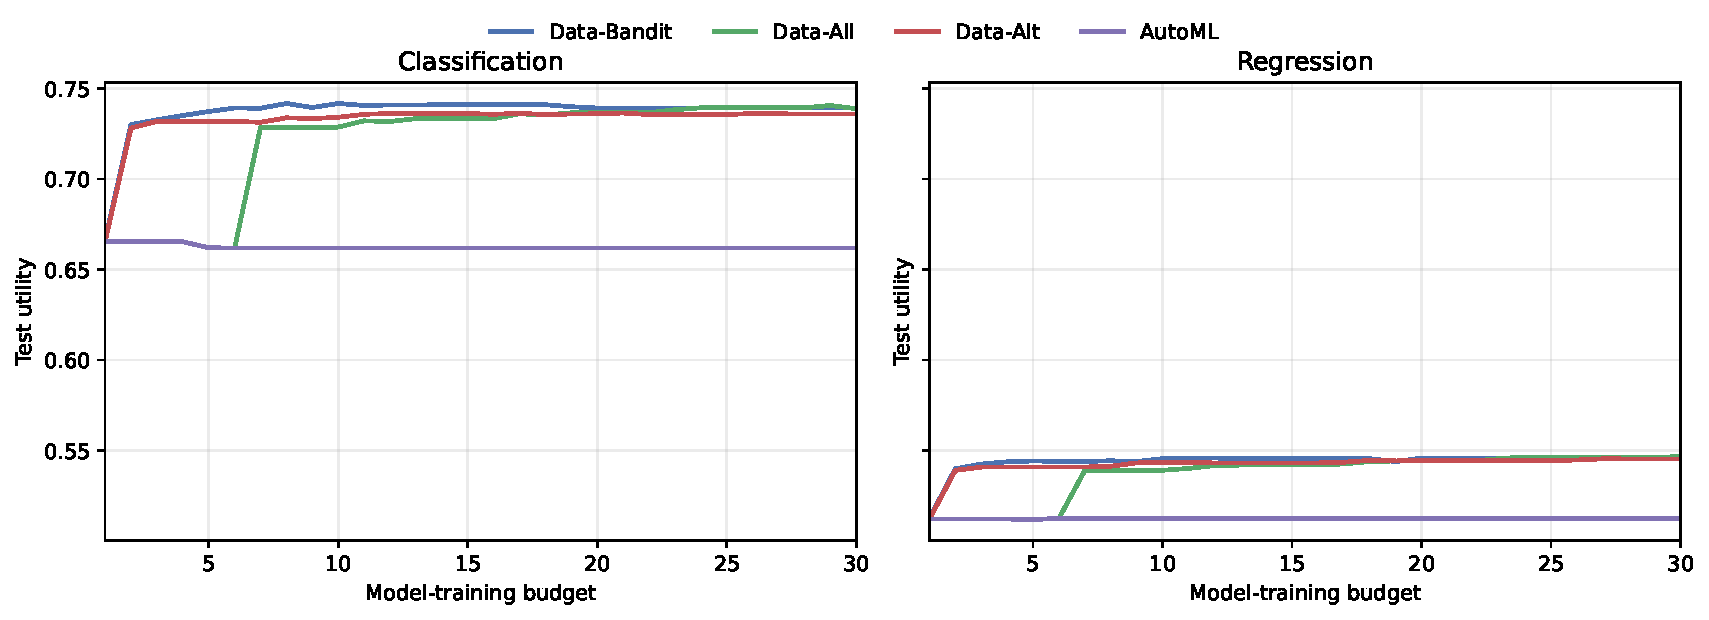
\includegraphics[width=0.94\linewidth]{rq1_discovery.pdf}
\vspace{-0.4em}
\begin{columns}[T,onlytextwidth]
\column{0.49\textwidth}
\begin{exampleblock}{相对 Data-All}
\small
\begin{itemize}
  \item 95\% 增益训练数：分类 $-30.3\%$，回归 $-27.5\%$
  \item AUC 配对差：$+0.00794$、$+0.00335$
  \item bootstrap 95\% 区间均不跨 0
\end{itemize}
\end{exampleblock}
\column{0.49\textwidth}
\begin{alertblock}{边界}
\small
Data-All 的 60 次预算末端效用仍最高；Data-Bandit 只落后 0.0012--0.0015。相对 Data-Alt 的 AUC 区间跨 0，不能声称稳定领先。
\end{alertblock}
\end{columns}
\end{frame}

\begin{frame}{RQ2：论文定价方法的 IS/OOS 复现}
\centering
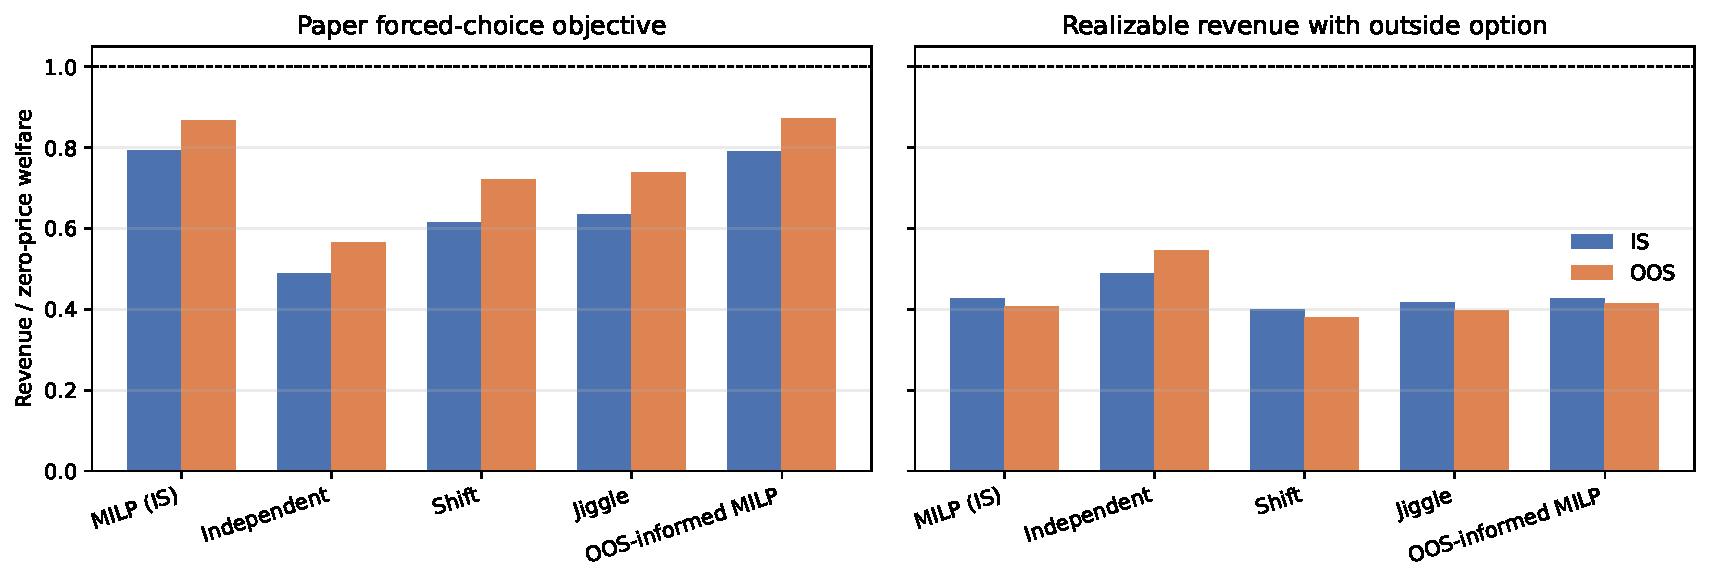
\includegraphics[width=0.88\linewidth]{rq2_paper_reproduction.pdf}
\vspace{-0.5em}
\begin{columns}[T,onlytextwidth]
\column{0.49\textwidth}
\begin{exampleblock}{论文强制购买指标}
\small MILP 的 IS 归一化收入为 $0.7926\pm0.0098$；Shift 优于 Independent，Jiggle 继续改善 Shift。
\end{exampleblock}
\column{0.49\textwidth}
\begin{alertblock}{自愿购买指标}
\small 本缩减设置下 Independent 的 OOS 实现收入最高，说明强制支付最优不等于可实现收入最优。
\end{alertblock}
\end{columns}
\end{frame}

\begin{frame}{RQ3：停止时间先验学习}
\centering
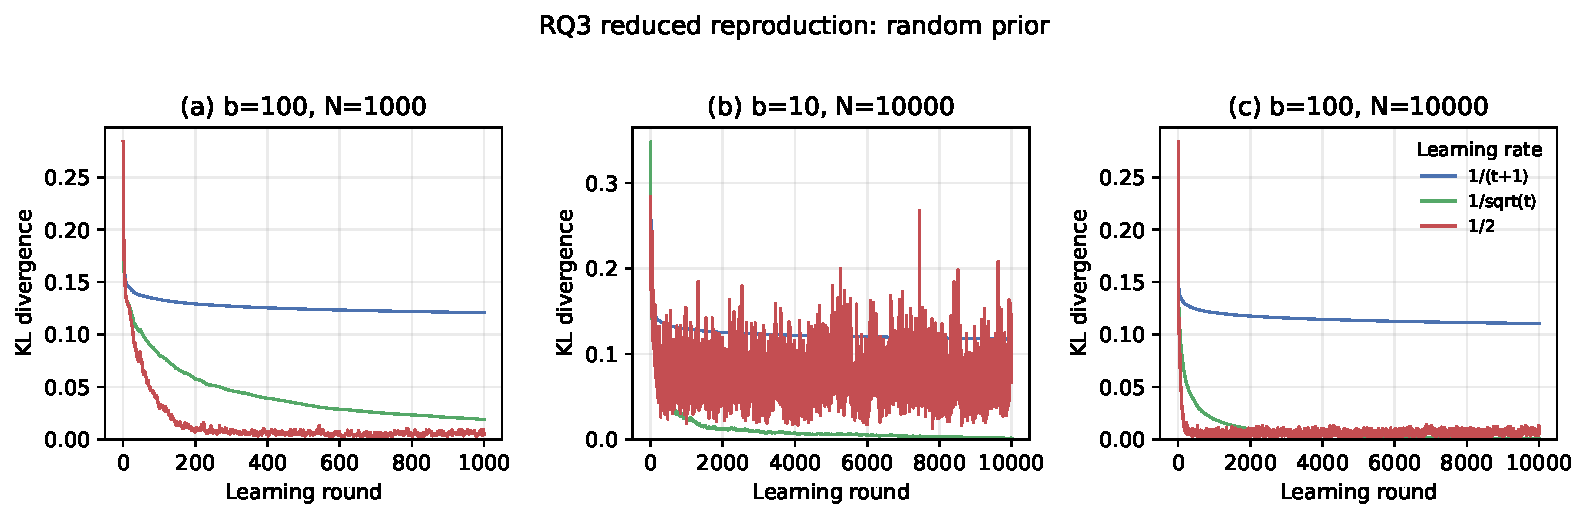
\includegraphics[height=0.48\textheight,keepaspectratio]{rq3_paper_reproduction.pdf}
\vspace{-0.5em}
\begin{columns}[T,onlytextwidth]
\column{0.49\textwidth}
\begin{exampleblock}{复现到的现象}
\small 大批量更平滑；激进学习率收敛更快；$1/\sqrt t$ 在速度和稳定性之间较均衡。
\end{exampleblock}
\column{0.49\textwidth}
\begin{alertblock}{必要前提}
\small 不同类型必须有可区分的停止分布。常数 $1/2$ 在批量 10 时振荡明显。
\end{alertblock}
\end{columns}
\end{frame}

\begin{frame}{发现的问题：正文“自愿购买”与 MILP 强制选择不一致}
\begin{alertblock}{论文程序中的关键约束}
\[
\sum_{q\in s}z(\theta,s,q)=1
\]
它强制每个类型在每条轨迹中购买一个模型。
\end{alertblock}
\begin{columns}[T,onlytextwidth]
\column{0.47\textwidth}
\begin{block}{真实理性行为}
如果
\[
\max_{q\in s}\{v^\theta(q)-x(q)\}<0,
\]
买家应当\textbf{不购买}。
\end{block}
\column{0.51\textwidth}
\begin{block}{原目标的偏差}
MILP 仍选择“亏损最少”的模型，并把正价格记作平台收入，因此可能偏好不可实施的高价曲线。
\end{block}
\end{columns}
\vspace{0.5em}
\centering
实验中强制目标为 0.4881，但允许退出后的训练实现收入仅 0.2687。
\end{frame}

\begin{frame}{改进一：加入个体理性外部选项}
增加虚拟选项 $\bot$：
\[
v^\theta(\bot)=x(\bot)=0,\qquad
q^*_{\mathrm{IR}}\in\arg\max_{q\in s\cup\{\bot\}}
\{v^\theta(q)-x(q)\}.
\]
\begin{columns}[T,onlytextwidth]
\column{0.48\textwidth}
\begin{exampleblock}{理论性质}
\begin{itemize}
  \item 每个类型--轨迹对都满足事后个体理性
  \item 可实现收入不再包含负效用买家的虚假支付
  \item 若原选择净效用处处非负，两目标完全一致
\end{itemize}
\end{exampleblock}
\column{0.50\textwidth}
\begin{block}{MILP 如何修改？}
\begin{itemize}
  \item 加入 $z(\theta,s,\bot)$
  \item 保留选择和为 1
  \item 固定外部选项价格、估值、支付为 0
  \item 或显式约束购买效用非负
\end{itemize}
\end{block}
\end{columns}
\end{frame}

\begin{frame}{改进二：先验偏移下的鲁棒 IR 定价}
候选先验集合 $\mathcal U$ 包含估计先验、均匀先验、低/高支付意愿偏移：
\[
\max_{x\ge0}\min_{\mu\in\mathcal U}
\E_{\theta\sim\mu,s\sim S}
[x(q^*_{\mathrm{IR}}(\theta,x,s))].
\]
\begin{table}
\centering
\small
\begin{tabular}{lrrr}
\toprule
机制 & IS 测试 & OOS 测试 & 主要定位\\
\midrule
Paper forced-choice & 0.2749 & 0.1106 & 原论文式目标\\
Independent & 0.3280 & 0.2169 & 边际定价基线\\
IR-aware & \textbf{0.3746} & 0.2436 & 同分布最优\\
Robust IR & 0.3367 & \textbf{0.2805} & 抗先验偏移\\
\bottomrule
\end{tabular}
\end{table}
\centering
Robust IR 相比普通 IR：OOS $+15.1\%$，代价是 IS $-10.1\%$。
\end{frame}

\begin{frame}{当前结论应该如何解读？}
\begin{columns}[T,onlytextwidth]
\column{0.49\textwidth}
\begin{exampleblock}{已有证据支持}
\begin{itemize}
  \item 论文核心停止与定价机制可实现
  \item 公开数据支持 Data-Bandit 的样本效率
  \item 缺少外部选项会系统性高估收入
  \item IR 修正提高可实现收入
  \item max--min 定价提高分布偏移稳定性
  \item 停止行为能够学习类型先验
\end{itemize}
\end{exampleblock}
\column{0.49\textwidth}
\begin{alertblock}{目前不能声称}
\begin{itemize}
  \item 不是原文 Figure 3--5 的逐点复现
  \item 尚未复现 69K NYC 数据池
  \item RQ1 是公开数据上的缩减替代实验
  \item RQ2/RQ3 是透明合成设置，不是原图逐点复制
  \item $|Q|=20$ 的开源 MILP 在时限内仍有大 gap
  \item 估值网格不是一般连续多质量定价的精确解
\end{itemize}
\end{alertblock}
\end{columns}
\end{frame}

\begin{frame}{当前重点与最终交付}
\begin{tikzpicture}[
  milestone/.style={rounded corners,draw=mainblue,thick,fill=mainblue!6,
                    minimum height=1.1cm,text width=2.65cm,align=center},
  done/.style={milestone,draw=goodgreen,fill=goodgreen!8},
  arrow/.style={-{Latex[length=2mm]},thick,draw=gray!70},
  node distance=0.45cm
]
\node[done] (m1) {v0.1--0.2\\机制、改进、报告、展示};
\node[done,right=of m1] (m2) {v0.3\\公开表格数据 + Exp3 / RQ1};
\node[done,right=of m2] (m3) {v0.4\\RQ2/RQ3 + 论文讲解};
\node[milestone,right=of m3] (m4) {v1.0\\讲懂、复现、报告与代码};
\draw[arrow] (m1)--(m2);
\draw[arrow] (m2)--(m3);
\draw[arrow] (m3)--(m4);
\end{tikzpicture}

\vspace{1.2em}
\begin{enumerate}
  \item 先把模型、算法、定理证明直觉和代码对应讲清楚；
  \item 固化 RQ1/RQ2/RQ3 的运行入口、原始表格和复现边界；
  \item 已有 MILP/IR 发现只做准确记录，暂缓大规模优化探索；
  \item 整合最终 PDF、展示、代码、Conda 环境与一键复现说明。
\end{enumerate}
\end{frame}

\begin{frame}{总结}
\begin{block}{论文贡献}
把数据增强、模型发现、最优停止和价格曲线统一到一个 AutoML 市场机制中。
\end{block}
\begin{exampleblock}{我们的复现工作}
\begin{enumerate}
  \item 实现并验证论文的停止 DP、经验定价与先验学习；
  \item 在公开数据上复现 RQ1，并完成多任务 RQ2、多设置 RQ3；
  \item 解释并实现 DP、MILP、先验学习和 Data-Bandit；
  \item 记录“自愿购买 vs. 强制选择”及有限价格上界边界；
  \item 建立 Conda、测试、原始结果、中文讲解和 PDF 工程。
\end{enumerate}
\end{exampleblock}
\vfill
\centering\Large 谢谢！欢迎提问
\end{frame}

\begin{frame}{附录：可复现入口}
\begin{itemize}
  \item 一键运行：\texttt{make all}
  \item 单元测试：\texttt{make test}
  \item 论文讲解：\texttt{docs/paper\_walkthrough.md}
  \item 原始结果：\texttt{results/paper\_experiments\_summary.json}
  \item RQ1 结果：\texttt{results/rq1\_summary.json}
  \item 表格结果：\texttt{results/tables/rq2\_paper\_summary.csv}
  \item 复现报告：\texttt{report/main.pdf}
  \item 课程展示：\texttt{slides/midterm.pdf}
  \item 当前版本：\texttt{v0.4.0}
\end{itemize}
\vspace{0.8em}
\small
参考论文：Y. Han, S. Padmanabha, S. Wang, Z. Huang, J. Zhao,
\emph{Optimal Pricing for Data-Augmented AutoML Marketplaces}.
\end{frame}

\end{document}
